\begin{name}
	{\tenchude}{\tendethi}{LỚP TOÁN THẦY PHÁT}{\thoigian}
\end{name}
\setcounter{ex}{0}\setcounter{bt}{0}
\Opensolutionfile{ans}[ans/ans-2-TT-31-KSCL-LeXoay-VinhPhuc-23]
\begin{ex}%[Đề thi KSCL lần 2 THPT Lê Xoay-Vĩnh Phúc năm 2023]%[Nguyễn Tấn Linh, dự án 12-EX-6-2023]%[2D3Y3-1]
Cho hai hàm số $f(x)$ và $g(x)$ liên tục trên $[a;b]$. Diện tích hình phẳng giới hạn bởi đồ thị của các hàm số $y=f(x),y=g(x)$ và các đường thẳng $x=a,x=b$ bằng
\choice
{$\left|\displaystyle\int\limits_a^b[f(x)-g(x)]\mathrm{\, d}x\right|$}
{\True $\displaystyle\int\limits_a^b|f(x)-g(x)|\mathrm{\, d}x$}
{$\displaystyle\int\limits_a^b[f(x)-g(x)]\mathrm{\, d}x$}
{$\displaystyle\int\limits_a^b|f(x)+g(x)|\mathrm{\, d}x$}
\loigiai
{
Diện tích hình phẳng giới hạn bởi đồ thị của các hàm số $y=f(x),y=g(x)$ và các đường thẳng $x=a,x=b$ là $S=\displaystyle\int\limits_a^b\left|f(x)-g(x)\right|\mathrm{\, d}x$.
}
\end{ex}

\begin{ex}%[Đề thi KSCL lần 2 THPT Lê Xoay-Vĩnh Phúc năm 2023]%[Nguyễn Tấn Linh, dự án 12-EX-6-2023]%[2D2Y5-1]
Tìm tập nghiệm $S$ của phương trình $5^{2x^2-x}=5$.
\choice
{$S=\{0;2\}$}
{$S=\left\{0;\dfrac{1}{2}\right\}$}
{\True $S=\left\{1;-\dfrac{1}{2}\right\}$}
{$S=\varnothing$}
\loigiai
{
Ta có $5^{2x^2-x}=5 \Leftrightarrow 2x^2-x=1 \Leftrightarrow \hoac{&x=1\\&x=-\dfrac{1}{2}.}$\\
Vậy tập nghiệm của phương trình là $S=\left\{1;-\dfrac{1}{2}\right\}$.
}
\end{ex}

\begin{ex}%[Đề thi KSCL lần 2 THPT Lê Xoay-Vĩnh Phúc năm 2023]%[Nguyễn Tấn Linh, dự án 12-EX-6-2023]%[2D3Y2-1]
Cho $\displaystyle\int\limits_1^2f(x)\mathrm{\, d}x=-3$ và $\displaystyle\int\limits_2^3f(x)\mathrm{\, d}x=4$. Khi đó $\displaystyle\int\limits_1^3f(x)\mathrm{\, d}x$ bằng
\choice
{$12$}
{$7$}
{$-12$}
{\True $1$}
\loigiai
{
Ta có $\displaystyle\int\limits_1^3f(x)\mathrm{\, d}x=\displaystyle\int\limits_1^2f(x)\mathrm{\, d}x+\displaystyle\int\limits_2^3f(x)\mathrm{\, d}x=-3+4=1$.
}
\end{ex}

\begin{ex}%[Đề thi KSCL lần 2 THPT Lê Xoay-Vĩnh Phúc năm 2023]%[Nguyễn Tấn Linh, dự án 12-EX-6-2023]%[2D3B2-1]
Cho $\displaystyle\int\limits_0^1f(x)\mathrm{\, d}x=2$ và $\displaystyle\int\limits_0^1g(x)\mathrm{\, d}x=5$, khi đó $\displaystyle\int\limits_0^1[5f(x)-g(x)]\mathrm{\, d}x$ bằng
\choice
{$1$}
{$3$}
{\True $5$}
{$-3$}
\loigiai
{
Ta có $\displaystyle\int\limits_0^1[5f(x)-g(x)]\mathrm{\, d}x=5\displaystyle\int\limits_0^1f(x)\mathrm{\, d}x-\displaystyle\int\limits_0^1g(x)\mathrm{\, d}x=5\cdot2-5=5$.
}
\end{ex}

\begin{ex}%[Đề thi KSCL lần 2 THPT Lê Xoay-Vĩnh Phúc năm 2023]%[Nguyễn Tấn Linh, dự án 12-EX-6-2023]%[2D3Y3-1]
	Cho hàm số $y=f(x)$ liên tục trên $\mathbb{R}$ và có đồ thị $(C)$ là đường cong như hình bên. Diện tích hình phẳng giới hạn bởi đồ thị $(C)$, trục hoành và hai đường thẳng $x=0,x=2$ là
\immini
{
\choice
{\True $\displaystyle\int\limits_0^1f(x)\mathrm{\, d}x-\displaystyle\int\limits_1^2f(x)\mathrm{\, d}x$}
{$\displaystyle\int\limits_0^1f(x)\mathrm{\, d}x+\displaystyle\int\limits_1^2f(x)\mathrm{\, d}x$}
{$\left|\displaystyle\int\limits_0^2f(x)\mathrm{\, d}x\right|$}
{$\displaystyle\int\limits_0^2f(x)\mathrm{\, d}x$}
}
{
\begin{tikzpicture}[line join = round, line cap = round,>=stealth,font=\footnotesize,scale=0.7,declare function={f(\x)=1/10*((\x)+2)^2*((\x)-1)*((\x)-3);}]
\def\xt{-3.5} \def\xp{4} \def\yd{-2} \def\yt{2}
\draw[->] (\xt,0)--(\xp,0) node[below]{$x$};
\draw[->] (0,\yd)--(0,\yt) node[left]{$y$};
\fill (0,0) circle (1.5pt) node[below left]{$O$};
\fill[pattern=north east lines] (0,0)--plot [domain=0:2](\x, {f(\x)})--(2,0);
\fill (1,0) circle (1.5pt) node[below]{$1$};
\fill (2,0) circle (1.5pt) node[above]{$2$};
\begin{scope}
\clip (\xt+0.1,\yd+0.1) rectangle (\xp-0.1,\yt-0.1);
\draw[samples=200,domain=\xt:\xp,smooth] plot (\x, {f(\x)});
\end{scope}
\end{tikzpicture}
}
\loigiai
{
Diện tích hình phẳng giới hạn bởi đồ thị $(C)$, trục hoành và hai đường thẳng $x=0,x=2$ là $S=\displaystyle\int\limits_0^2\left|f(x)\right|\mathrm{\, d}x=\displaystyle\int\limits_0^1\left|f(x)\right|\mathrm{\, d}x+\displaystyle\int\limits_1^2\left|f(x)\right|\mathrm{\, d}x=\displaystyle\int\limits_0^1f(x)\mathrm{\, d}x-\displaystyle\int\limits_1^2f(x)\mathrm{\, d}x$.
}
\end{ex}

\begin{ex}%[Đề thi KSCL lần 2 THPT Lê Xoay-Vĩnh Phúc năm 2023]%[Nguyễn Tấn Linh, dự án 12-EX-6-2023]%[1D2Y2-1]
Có bao nhiêu cách xếp 4 học sinh nam và 5 học sinh nữ thành 1 hàng dọc?
\choice
{\True 9!}
{$9$}
{$20$}
{$4!\cdot 5$!}
\loigiai
{
Có tổng cộng $9$ học sinh.\\
Mỗi cách xếp $9$ học sinh thành $1$ hàng dọc là một hoán vị của $9$ học sinh.\\
Vậy ta có $9!$ cách xếp $9$ học sinh thành 1 hàng dọc.
}
\end{ex}

\begin{ex}%[Đề thi KSCL lần 2 THPT Lê Xoay-Vĩnh Phúc năm 2023]%[Nguyễn Tấn Linh, dự án 12-EX-6-2023]%[2D2Y1-2]
Cho $x,y>0$ và $\alpha,\beta\in\mathbb{R}$. Khẳng định nào dưới đây là \textbf{sai}?
\choice
{$x^{\alpha}\cdot x^{\beta}=x^{\alpha+\beta}$}
{$\left(x^{\alpha}\right)^{\beta}=x^{\alpha\beta}$}
{\True $x^{\alpha}+y^{\alpha}=(x+y)^{\alpha}$}
{$(x y)^{\alpha}=x^{\alpha}\cdot y^{\alpha}$}
\loigiai
{
Khẳng định $x^{\alpha}+y^{\alpha}=(x+y)^{\alpha}$ sai vì $1^2+2^2\ne (1+2)^2$.
}
\end{ex}

\begin{ex}%[Đề thi KSCL lần 2 THPT Lê Xoay-Vĩnh Phúc năm 2023]%[Nguyễn Tấn Linh, dự án 12-EX-6-2023]%[2D1B2-2]
Cho hàm số $f(x)$ liên tục trên $\mathbb{R}$ và có bảng xét dấu của $f'(x)$ như sau
\begin{center}

\begin{tikzpicture}
\tkzTabInit[lgt=1.2,espcl=2,deltacl=0.5]
{$x$ /0.7, $f'(x)$ /0.7}
{$-\infty$,$-1$,$0$,$1$,$2$,$+\infty$}
\tkzTabLine{ ,+,$0$,-,$0$,+,d,-,$0$,-, }
\end{tikzpicture}
\end{center}
Số điểm cực trị của hàm số đã cho là
\choice
{$1$}
{\True $3$}
{$4$}
{$2$}
\loigiai
{
Ta có $f(x)$ liên tục trên $\mathbb{R}$ và $f'(x)$ đổi dấu khi $x$ đi qua $x_1=-1, x_2=0, x_3=1$ nên hàm số $f(x)$ có 3 điểm cực trị.
}
\end{ex}

\begin{ex}%[Đề thi KSCL lần 2 THPT Lê Xoay-Vĩnh Phúc năm 2023]%[Nguyễn Tấn Linh, dự án 12-EX-6-2023]%[1D2Y2-1]
Cho số tự nhiên dương $n$. Mệnh đề nào sau đây là \textbf{sai}?
\choice
{$\mathrm{C}_{n+1}^0=1$}
{$\mathrm{C}_n^n=1$}
{$\mathrm{C}_n^{n-1}=n$}
{\True $\mathrm{C}_n^1=n+1$}
\loigiai
{
Mệnh đề $\mathrm{C}_n^1=n+1$ sai vì $\mathrm{C}_n^1=n$.
}
\end{ex}

\begin{ex}%[Đề thi KSCL lần 2 THPT Lê Xoay-Vĩnh Phúc năm 2023]%[Nguyễn Tấn Linh, dự án 12-EX-6-2023]%[2D1Y4-1]
Tiệm cận ngang của đồ thị hàm số $y=\dfrac{2x+2}{x-1}$ là
\choice
{$x=-1$}
{\True $y=2$}
{$x=1$}
{$y=1$}
\loigiai
{
Ta có $\lim\limits_{x \to +\infty}y=\lim\limits_{x \to +\infty}\dfrac{2x+2}{x-1}=2$. Do đó tiệm cận ngang của đồ thị hàm số đã cho là $y=2$.
}
\end{ex}

\begin{ex}%[Đề thi KSCL lần 2 THPT Lê Xoay-Vĩnh Phúc năm 2023]%[Nguyễn Tấn Linh, dự án 12-EX-6-2023]%[2H2Y2-1]
Diện tích của một mặt cầu bằng $16\pi($$ cm^2)$. Bán kính của mặt cầu đó là
\choice
{$8$ cm}
{$6$ cm}
{$4$ cm}
{\True $2$ cm}
\loigiai
{
Gọi $R$ là bán kính mặt cầu.\\
Ta có diện tích mặt cầu là $S=4\pi R^2 \Rightarrow 16\pi =4\pi R^2 \Leftrightarrow R=2$.
}
\end{ex}

\begin{ex}%[Đề thi KSCL lần 2 THPT Lê Xoay-Vĩnh Phúc năm 2023]%[Nguyễn Tấn Linh, dự án 12-EX-6-2023]%[2H3Y1-1]
Trong không gian với hệ trục tọa độ $O x y z$, cho hai điểm $A(0;1;-2)$ và $B(3;-1;1)$. Tìm tọa độ trung điểm $M$ của đoạn thẳng $AB$.
\choice
{\True $M\left(\dfrac{3}{2};0;\dfrac{-1}{2}\right)$}
{$M(3;-2;3)$}
{$M\left(\dfrac{3}{2};-1;\dfrac{3}{2}\right)$}
{$M\left(\dfrac{-3}{2};1;\dfrac{-3}{2}\right)$}
\loigiai
{
Ta có $M$ là trung điểm của đoạn thẳng $AB$ nên\\
$\heva{&x_M=\dfrac{x_A+x_B}{2}=\dfrac{0+3}{2}=\dfrac{3}{2}\\&y_M=\dfrac{y_A+y_B}{2}=\dfrac{1-1}{2}=0\\&z_M=\dfrac{z_A+z_B}{2}=\dfrac{-2+1}{2}=-\dfrac{1}{2}}\\
\Rightarrow M\left(\dfrac{3}{2};0;-\dfrac{1}{2}\right)$.
}
\end{ex}

\begin{ex}%[Đề thi KSCL lần 2 THPT Lê Xoay-Vĩnh Phúc năm 2023]%[Nguyễn Tấn Linh, dự án 12-EX-6-2023]%[2H2Y2-3]
Thể tích khối cầu nội tiếp hình lập phương có cạnh bằng 2 là
\choice
{$4\pi$}
{$8\pi$}
{\True $\dfrac{4\pi}{3}$}
{$\dfrac{32\pi}{3}$}
\loigiai
{
Bán kính khối cầu đã cho là $R=\dfrac{2}{2}=1$.\\
Thể tích khối cầu đã cho là $V=\dfrac{4}{3}\pi R^3=\dfrac{4\pi}{3}$.
}
\end{ex}

\begin{ex}%[Đề thi KSCL lần 2 THPT Lê Xoay-Vĩnh Phúc năm 2023]%[Nguyễn Tấn Linh, dự án 12-EX-6-2023]%[2D1Y5-1]
\immini
{
Đường cong ở hình bên là đồ thị của hàm số $y=\dfrac{a x+b}{c x+d}$ với $a,b,c,d$ là các số thực. Mệnh đề nào dưới đây đúng?
\choice
{$y'<0,\forall x\ne 1$}
{$y'>0,\forall x\ne 1$}
{$y'>0,\forall\ne 2$}
{\True $y'<0,\forall x\ne 2$}
}
{
\begin{tikzpicture}[line join = round, line cap = round,>=stealth,font=\footnotesize,scale=0.4,declare function={f(\x)=(\a*\x+(\b))/(\c*\x+(\d));}]
\def\xt{-3} \def\xp{7} \def\yd{-4} \def\yt{6}
\def\a{1}
\def\b{1}
\def\c{1}
\def\d{-2}
\draw[->] (\xt,0)--(\xp,0) node[below]{$x$};
\draw[->] (0,\yd)--(0,\yt) node[left]{$y$};
\fill (0,0) circle (1.5pt) node[above left]{$O$};
\fill (0,1) circle (1.5pt) node[above left]{$1$};
\fill (2,0) circle (1.5pt) node[below right]{$2$};
\begin{scope}
\clip (\xt+0.1,\yd+0.1) rectangle (\xp-0.1,\yt-0.1);
\pgfmathsetmacro{\tcn}{(\a)/(\c)}
\pgfmathsetmacro{\tcd}{-(\d)/(\c)}
\draw[dashed] (\xt,\tcn)--(\xp,\tcn) (\tcd,\yd)--(\tcd,\yt);
\draw[samples=150,smooth,domain={\tcd+0.01}:\xp] plot(\x,{f(\x)});
\draw[samples=150,smooth,domain=\xt:{\tcd-0.01}] plot(\x,{f(\x)});
\end{scope}
\end{tikzpicture}
}
\loigiai
{
Dựa vào đồ thị, ta thấy hàm số đã cho nghịch biến trên $(-\infty;2)$ và $(2;+\infty)$. Do đó $y'<0,\forall x\ne2$.
}
\end{ex}
\begin{ex}%[Đề thi KSCL lần 2 THPT Lê Xoay-Vĩnh Phúc năm 2023]%[Nguyễn Tấn Linh, dự án 12-EX-6-2023]%[2H3Y2-6]
Trong không gian với hệ trục tọa độ $O x y z$, khoảng cách từ điểm $A(3;1;-2)$ đến mặt phẳng $z=0$ bằng
\choice
{$\sqrt{5}$}
{$\sqrt{14}$}
{\True $2$}
{$3$}
\loigiai
{
Khoảng cách từ điểm $A$ đến mặt phẳng $z=0$ là $\mathrm{d}=\dfrac{|-2|}{\sqrt{1^2}}=2$.
}
\end{ex}

\begin{ex}%[Đề thi KSCL lần 2 THPT Lê Xoay-Vĩnh Phúc năm 2023]%[Nguyễn Tấn Linh, dự án 12-EX-6-2023]%[2H3Y1-3]
Trong không gian với hệ tọa độ $O x y z$, hỏi trong các phương trình sau phương trình nào là phương trình của mặt cầu?
\choice
{\True $x^2+y^2+z^2-2x+4z-1=0$}
{$x^2+y^2+z^2+2x y-4y+4z-1=0$}
{$x^2+y^2+z^2-2x+2y-4z+8=0$}
{$x^2+z^2+3x-2y+4z-1=0$}
\loigiai
{
Phương trình $(S):x^2+y^2+z^2-2ax-2by-2cz+d=0$ là phương trình mặt cầu khi và chỉ khi $a^2+b^2+c^2-d>0$.\\
Vậy phương trình $x^2+y^2+z^2-2x+4z-1=0$ là phương trình mặt cầu.
}
\end{ex}

\begin{ex}%[Đề thi KSCL lần 2 THPT Lê Xoay-Vĩnh Phúc năm 2023]%[Nguyễn Tấn Linh, dự án 12-EX-6-2023]%[1H3B2-3]
\immini
{
Cho hình lập phương $ABCD.EFGH$. Góc giữa hai đường thẳng $AF$ và $EG$ bằng
\choice
{$0^\circ$}
{\True $60^\circ$}
{$90^\circ$}
{$30^\circ$}
}
{
\begin{tikzpicture}[line join=round,line cap=round,font=\footnotesize,scale=.7]
\def\ngang{3}
\def \doc{3}
\coordinate (E) at (0,0);
\coordinate (F) at (1,1.2);
\coordinate (H) at (\ngang,0);
\coordinate (G) at ($(H)-(E)+(F)$);
\coordinate (B) at ($(F)+(90:\doc)$);
\coordinate (A) at ($(E)-(F)+(B)$);
\coordinate (D) at ($(H)-(F)+(B)$);
\coordinate (C) at ($(G)-(F)+(B)$);
\draw (A)--(E)--(H)--(G)--(C)--(B)--(A)--(D)--(C) (H)--(D);
\draw[dashed] (F)--(G) (B)--(F)--(E) (A)--(F) (E)--(G);
\foreach \diem/\goc in {F/160,E/-90,H/-90,G/0,A/180,D/-25,C/90,B/90} \fill[black](\diem) circle (1pt) ($(\diem)+(\goc:3mm)$) node{$\diem$};
\end{tikzpicture}
}
\loigiai
{
Ta có $AF\parallel DG$ nên góc giữa $AF$ và $EG$ là góc giữa $DG$ và $EG$ và bằng $\widehat{DGE}$.\\
Lại có $DE=DG=EG$ nên tam giác $DEG$ đều. Suy ra $\widehat{DGE}=60^{\circ}$.
}
\end{ex}
\begin{ex}%[Đề thi KSCL lần 2 THPT Lê Xoay-Vĩnh Phúc năm 2023]%[Nguyễn Tấn Linh, dự án 12-EX-6-2023]%[2H3Y1-3]
Trong không gian với hệ tọa độ $O x y z$, mặt cầu $(S)\colon  x^2+y^2+z^2-6x+4y-2z-2=0$ có bán kính là
\choice
{$2$}
{\True $4$}
{$2\sqrt{3}$}
{$\sqrt{2}$}
\loigiai
{
Mặt cầu $(S)\colon x^2+y^2+z^2-6x+4y-2z-2=0$ có tâm $I(3;-2;1)$ và bán kính $R=4$.
}
\end{ex}

\begin{ex}%[Đề thi KSCL lần 2 THPT Lê Xoay-Vĩnh Phúc năm 2023]%[Nguyễn Tấn Linh, dự án 12-EX-6-2023]%[2D3Y1-1]
Họ nguyên hàm của hàm số $f(x)=\cos x$ là
\choice
{$-\cos x+C$}
{$\cos x+C$}
{\True $\sin x+C$}
{$-\sin x+C$}
\loigiai
{
Ta có $\displaystyle\int f(x)\mathrm{\, d}x=\displaystyle\int \cos x\mathrm{\, d}x=\sin x+C$.
}
\end{ex}

\begin{ex}%[Đề thi KSCL lần 2 THPT Lê Xoay-Vĩnh Phúc năm 2023]%[Nguyễn Tấn Linh, dự án 12-EX-6-2023]%[2H2Y1-1]
Một hình trụ có bán kính đáy $r=5$ cm, chiều cao $h=7$ cm. Thể tích của hình trụ đó bằng
\choice
{\True $175\pi$ (cm$^3$)}
{$\dfrac{175}{3}\pi$ (cm$^3$)}
{$70\pi$ (cm$^3$)}
{$S=35\pi$ (cm$^3$)}
\loigiai
{
Thể tích hình trụ là $V=\pi r^2h=\pi\cdot 5^2\cdot 7=175\pi$ (cm$^3$).
}
\end{ex}

\begin{ex}%[Đề thi KSCL lần 2 THPT Lê Xoay-Vĩnh Phúc năm 2023]%[Nguyễn Tấn Linh, dự án 12-EX-6-2023]%[2D2Y3-2]
Cho hai số dương $a,b$ $(a\ne 1)$. Mệnh đề nào dưới đây \textbf{sai}?
\choice
{$\log_a a^{\alpha}=\alpha$}
{$a^{\log_a b}=b$}
{$\log_a 1=0$}
{\True $\log_a a=2a$}
\loigiai
{
Mệnh đề sai là $\log_a a=2a$, vì $\log_aa=1$ với mọi $a>0,a\ne 1$.
}
\end{ex}

\begin{ex}%[Đề thi KSCL lần 2 THPT Lê Xoay-Vĩnh Phúc năm 2023]%[Nguyễn Tấn Linh, dự án 12-EX-6-2023]%[2D2Y4-1]
Tập xác định của hàm số $y=\ln (3x-6)$ là
\choice
{\True $(2;+\infty)$}
{$\mathbb{R}\setminus\{2\}$}
{$(-\infty;2)$}
{$[2;+\infty)$}
\loigiai
{
Hàm số xác định khi $3x-6>0\Leftrightarrow x>2$.\\
Vậy tập xác định $\mathscr{D}=(2;+\infty)$.
}
\end{ex}

\begin{ex}%[Đề thi KSCL lần 2 THPT Lê Xoay-Vĩnh Phúc năm 2023]%[Nguyễn Tấn Linh, dự án 12-EX-6-2023]%[2H3Y3-1]
Trong không gian $O x y z$, cho đường thẳng $d\colon\dfrac{x-3}{2}=\dfrac{y-1}{-2}=\dfrac{z+1}{3}$. Véc-tơ nào dưới đây là một véc-tơ chỉ phương của $d$?
\choice
{\True $\overrightarrow{u_4}=(2;-2;3)$}
{$\overrightarrow{u_1}=(-3;-1;1)$}
{$\overrightarrow{u_3}=(3;1;-1)$}
{$\overrightarrow{u_2}=(2;2;3)$}
\loigiai
{
Véc-tơ $\overrightarrow{u_4}=(2;-2;3)$ là một véc-tơ chỉ phương của $d$.
}
\end{ex}

\begin{ex}%[Đề thi KSCL lần 2 THPT Lê Xoay-Vĩnh Phúc năm 2023]%[Nguyễn Tấn Linh, dự án 12-EX-6-2023]%[1D3B4-1]
Dãy số nào sau đây \textbf{không} phải là cấp số nhân?
\choice
{$1;2;4;8;16$}
{\True $1;2;3;4;5$}
{$1;-1;1;-1;1$}
{$1;-2;4;-8;16$}
\loigiai
{
Dãy số $1;2;3;4;5$ không là cấp số nhân vì $\dfrac{2}{1}\ne \dfrac{3}{2}$.
}
\end{ex}

\begin{ex}%[Đề thi KSCL lần 2 THPT Lê Xoay-Vĩnh Phúc năm 2023]%[Nguyễn Tấn Linh, dự án 12-EX-6-2023]%[2H2Y1-2]
Cho hình trụ có bán kính đáy bằng 6, đường cao bằng 8. Diện tích xung quanh của hình trụ đó bằng
\choice
{$60\pi$}
{$48\pi$}
{\True $96\pi$}
{$120\pi$}
\loigiai
{
Diện tích xung quanh $S_{\text{xq}}=2\pi rh=96\pi$.
}
\end{ex}

\begin{ex}%[Đề thi KSCL lần 2 THPT Lê Xoay-Vĩnh Phúc năm 2023]%[Nguyễn Tấn Linh, dự án 12-EX-6-2023]%[2H3Y2-1]
Trong không gian $O x y z$, cho 2 véc-tơ $\overrightarrow{u}=(5;4;2)$ và $\overrightarrow{v}=(1;2;4)$. Tích có hướng $[\overrightarrow{u},\overrightarrow{v}]$ là?
\choice
{$(-12;18;-6)$}
{$(12;-18;6)$}
{$(12;18;6)$}
{\True $(12;-18;-6)$}
\loigiai
{
Ta có $[\overrightarrow{u},\overrightarrow{v}]=(12;-18;-6)$.
}
\end{ex}

\begin{ex}%[Đề thi KSCL lần 2 THPT Lê Xoay-Vĩnh Phúc năm 2023]%[Nguyễn Tấn Linh, dự án 12-EX-6-2023]%[2D1B1-1]
Hàm số $y=-x^4+2x^2+1$ đồng biến trên khoảng nào dưới đây?
\choice
{$(0;+\infty)$}
{\True $(-\infty;-1)$}
{$(1;+\infty)$}
{$(-\infty;0)$}
\loigiai
{
Tập xác định $\mathscr{D}=\mathbb{R}$.\\
Ta có $y'=-4x^3+4x$, $y'=0\Leftrightarrow \hoac{& x=0 \\ & x=1 \\ & x=-1.}$\\
Bảng biến thiên
\begin{center}

\begin{tikzpicture}[>=stealth]
\tkzTabInit[nocadre=false,lgt=1,espcl=2,deltacl=0.5]{$x$/.7 ,$y'$/.7,$y$/2}
{$-\infty$ , $-1$ , $0$ , $1$ , $+\infty$}
\tkzTabLine{ , + , $0$ , - , $0$ , + , $0$ , - , }
\tkzTabVar{-/$-\infty$ , +/$2$, -/$1$ , +/$2$ , -/$-\infty$}
\end{tikzpicture}
\end{center}
Từ bảng biến thiên, suy ra hàm số đồng biến trên khoảng $(-\infty;-1)$.
}
\end{ex}

\begin{ex}%[Đề thi KSCL lần 2 THPT Lê Xoay-Vĩnh Phúc năm 2023]%[Nguyễn Tấn Linh, dự án 12-EX-6-2023]%[2H3Y2-2]
Trong không gian $O x y z$, mặt phẳng $(P)\colon 2x+y-3=0$ có một véc-tơ pháp tuyến là
\choice
{\True $\overrightarrow{n}=(2;1;0)$}
{$\overrightarrow{n}=(4;1;-3)$}
{$\overrightarrow{n}=(2;-3;0)$}
{$\overrightarrow{n}=(2;1;-3)$}
\loigiai
{
Mặt phẳng $(P)\colon 2x+y-3=0$ có một véc-tơ pháp tuyến là $\overrightarrow{n}=(2;1;0)$.
}
\end{ex}

\begin{ex}%[Đề thi KSCL lần 2 THPT Lê Xoay-Vĩnh Phúc năm 2023]%[Nguyễn Tấn Linh, dự án 12-EX-6-2023]%[2D1G5-3]
\immini
{
Cho hàm số $y=f(x)$ liên tục trên $\mathbb{R}$ có đồ thị như hình vẽ. Giá trị lớn nhất của hàm số $y=f(x)$ trên đoạn $[-1;3]$ bằng
\choice
{$-1$}
{Không tồn tại}
{$0$}
{\True $2$}
}
{
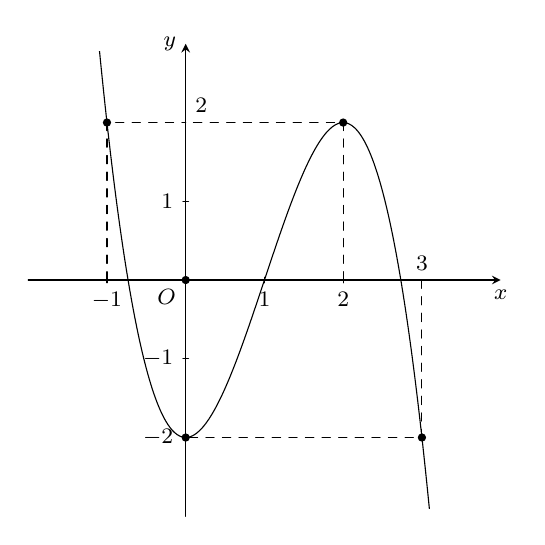
\begin{tikzpicture}[line join = round, line cap = round,>=stealth,font=\footnotesize,scale=1,declare function={f(\x)=\a*(\x)^3+(\b)*(\x)^2+(\c)*\x+(\d);}]
\def\xt{-2} \def\xp{4} \def\yd{-3} \def\yt{3}
\def\a{-1}
\def\b{3}
\def\c{0}
\def\d{-2}
\draw[->] (\xt,0)--(\xp,0) node[below]{$x$};
\draw[->] (0,\yd)--(0,\yt) node[left]{$y$};
\fill (0,0) circle (1.5pt) node[below left]{$O$};
\foreach \x in {-1,1,2} \draw[thin] (\x,1pt)--(\x,-1pt) node [below] {$\x$};
\foreach \y in {-2,-1,1} \draw[thin] (1pt,\y)--(-1pt,\y) node [left] {$\y$};
\draw[dashed] (-1,0)--(-1,2)--(0,2) node[above right]{$2$};
\draw[dashed] (2,0)--(2,2)--(0,2);
\draw[dashed] (3,0) node[above]{$3$}--(3,-2)--(0,-2);
\foreach \x/\y in {-1/2,2/2,0/-2,3/-2}\fill (\x,\y) circle (1.5pt);
\begin{scope}
\clip (\xt+0.1,\yd+0.1) rectangle (\xp-0.1,\yt-0.1);
\draw[samples=150,smooth,domain=\xt:\xp] plot(\x,{f(\x)});
\end{scope}
\end{tikzpicture}
}
\loigiai
{
Từ đồ thị, ta có $\max\limits_{[-1;3]} y=2$.
}
\end{ex}
\begin{ex}%[Đề thi KSCL lần 2 THPT Lê Xoay-Vĩnh Phúc năm 2023]%[Nguyễn Tấn Linh, dự án 12-EX-6-2023]%[2H2Y1-2]
Gọi $l$, $h$, $r$ lần lượt là độ dài đường sinh, chiều cao và bán kính mặt đáy của hình nón. Diện tích xung quanh $S_{\text{x q}}$ của hình nón là
\choice
{$S_{\text{xq}}=\pi r h$}
{$S_{\text{xq}}=\pi r l$}
{$S_{\text{xq}}=\dfrac{1}{3}\pi r^2h$}
{\True $S_{\text{xq}}=2\pi r l$}
\loigiai
{
Ta có $S_{\text{xq}}=2\pi r l$.
}
\end{ex}

\begin{ex}%[Đề thi KSCL lần 2 THPT Lê Xoay-Vĩnh Phúc năm 2023]%[Nguyễn Tấn Linh, dự án 12-EX-6-2023]%[2H3B3-2]
Trong không gian $O x y z$, đường thẳng $\Delta$ đi qua $M(1;-2;2),N(3;1;0)$ có phương trình là
\choice
{$\heva{&x=3+2t\\&y=1+3t\\&z=2t}$}
{$\heva{&x=1+2t\\&y=-2+1t\\&z=2-2t}$}
{$\heva{&x=1+2t\\&y=-2-3t\\&z=2+2t}$}
{\True $\heva{&x=3-2t\\&y=1-3t\\&z=2t}$}
\loigiai
{
Ta có $\overrightarrow{MN}=(2;3;-2)$. Suy ra véc-tơ chỉ phương của $\Delta$ là $\overrightarrow{u}=(-2;-3;2)$.\\
Phương trình đường thẳng $\Delta\colon \heva{&x=3-2t\\&y=1-3t\\&z=2t.}$
}
\end{ex}

\begin{ex}%[Đề thi KSCL lần 2 THPT Lê Xoay-Vĩnh Phúc năm 2023]%[Nguyễn Tấn Linh, dự án 12-EX-6-2023]%[2H2K1-2]
Cho hình nón có chiều cao bằng $6$, đường kính đáy bằng 20. Một thiết diện đi qua đỉnh của hình nón có khoảng cách từ tâm của đáy đến mặt phẳng chứa thiết diện là $4,8$. Tính diện tích $S$ của thiết diện đó.
\choice
{$S=160\sqrt{3}$}
{$S=80\sqrt{3}$}
{$S=120$}
{\True $S=60$}
\loigiai
{
\immini
{
Giả sử hình nón đỉnh $S$, tâm đường tròn đáy là $O$ và thiết diện qua đỉnh của hình nón là tam giác $SAB$. Ta có $SO=6$ và $OA=OB=10$.\\
Gọi $K$ là trung điểm của $AB$ và $H$ là hình chiếu của $O$ lên $SK$.\\
Ta suy ra $OK\perp AB$ và $\mathrm{d}(O,(SAB))=OH=4,8$.\\
Ta có $\dfrac{1}{OH^2}=\dfrac{1}{SO^2}+\dfrac{1}{OK^2}\Rightarrow OK=8$.\\
Tam giác $OKB$ vuông tại $K$ nên $KB=\sqrt{OB^2-OK^2}=6$, do đó $AB=2KB=12$.\\
Tam giác $SKO$ vuông tại $O$ nên $SK=\sqrt{SO^2+OK^2}=10$.\\
Diện tích tam giác $SAB$ là $S=\dfrac{1}{2}SK\cdot AB=\dfrac{1}{2}\cdot 10\cdot 12=60$.
}
{
\begin{tikzpicture}[scale=1, font=\footnotesize, line join=round, line cap=round, >=stealth]
\def\x{3} % Bán kính trụ lớn
\pgfmathsetmacro{\y}{\x/4} % Bán kính trục bé
\def\h{5} % Chiều cao
\coordinate (A1) at (\x,0); % Điểm bên phải
\coordinate[label=right:$O$] (O) at (0,0);
\coordinate[label=above left:$S$] (S) at (0,\h);
\coordinate[label=above right:$A$] (A) at ($(O)+(145:\x cm and \y cm)$);
\coordinate[label=below:$B$] (B) at ($(O)+(-100:\x cm and \y cm)$);
\coordinate[label=left:$K$] (K) at ($(A)!0.5!(B)$);
\coordinate[label=left:$H$] (H) at ($(S)!0.6!(K)$);
\draw (A1) arc (0:-180:{\x} and {\y})--(S)--cycle (S)--(B);
\draw[dashed] (S)--(O) (A1) arc (0:180:{\x} and {\y}) (K)--(S)--(A)--(B) (K)--(O)--(H) (A)--(O)--(B);
\foreach \x/\dinh/\y in {O/K/B, O/H/K, S/O/K} \draw[fill = gray!50] ($(\dinh)!5pt!(\x)$)--($(\dinh)!5pt!(\x)+(\dinh)!5pt!(\y)-(\dinh)$)--($(\dinh)!5pt!(\y)$)--(\dinh)--cycle;
\foreach \diem in {S,O,A,B,K,H}\fill (\diem)circle(1.5pt);
\end{tikzpicture}
}
}
\end{ex}

\begin{ex}%[Đề thi KSCL lần 2 THPT Lê Xoay-Vĩnh Phúc năm 2023]%[Nguyễn Tấn Linh, dự án 12-EX-6-2023]%[2D1K3-1]
Tổng giá trị lớn nhất và giá trị nhỏ nhất của hàm số $y=\dfrac{x+m}{x+1}$ trên $[1;2]$ bằng $8$ ($m$ là tham số thực). Khẳng định nào sau đây đúng?
\choice
{$0<m<4$}
{$4<m<8$}
{\True $8<m<10$}
{$m>10$}
\loigiai
{
Vì hàm số đã cho liên tục trên đoạn $[1;2]$ và có đạo hàm không đổi dấu trên đoạn đó, nên tổng giá trị lớn nhất và giá trị nhỏ nhất của hàm số trên đoạn $[1;2]$ chính là $y(1)+y(2)$.\\
Ta có $y(1)+y(2)=8\Leftrightarrow \dfrac{1+m}{2}+\dfrac{2+m}{3}=8\Leftrightarrow m=\dfrac{41}{5}\in (8;10)$.
}
\end{ex}

\begin{ex}%[Đề thi KSCL lần 2 THPT Lê Xoay-Vĩnh Phúc năm 2023]%[Nguyễn Tấn Linh, dự án 12-EX-6-2023]%[2D2B5-2]
Cho phương trình $\log_2(2x-1)^2=2\log_2(x-2)$. Số nghiệm thực của phương trình là
\choice
{$1$}
{$2$}
{\True $0$}
{$3$}
\loigiai
{
Điều kiện $\heva{& 2x-1\ne 0 \\ & x-2>0}\Leftrightarrow \heva{& x\ne \dfrac{1}{2} \\ & x>2.}$\\
Ta có
\begin{align*}
\log_2(2x-1)^2=2\log_2(x-2)&\Leftrightarrow |2x-1|=x-2\\
&\Leftrightarrow \heva{& x-2\ge 0 \\ & \hoac{& 2x-1=x-2 \\ & 2x-1=2-x}}\\
&\Leftrightarrow \heva{& x\ge 2 \\ & \hoac{& x=-1&&\text{(loại)} \\ & x=1&&\text{(loại)}.}}
\end{align*}
Vậy số nghiệm của phương trình đã cho là $0$.
}
\end{ex}

\begin{ex}%[Đề thi KSCL lần 2 THPT Lê Xoay-Vĩnh Phúc năm 2023]%[Nguyễn Tấn Linh, dự án 12-EX-6-2023]%[2D2B6-2]
Tập nghiệm $S$ của bất phương trình $5^{x+2}<\left(\dfrac{1}{25}\right)^{-x}$ là
\choice
{$S=(1;+\infty)$}
{$S=(-\infty;1)$}
{\True $S=(2;+\infty)$}
{$S=(-\infty;2)$}
\loigiai
{
Ta có $5^{x+2}<\left(\dfrac{1}{25}\right)^{-x}\Leftrightarrow 5^{x+2}<5^{2x}\Leftrightarrow x+2<2x\Leftrightarrow x>2$.
}
\end{ex}

\begin{ex}%[Đề thi KSCL lần 2 THPT Lê Xoay-Vĩnh Phúc năm 2023]%[Nguyễn Tấn Linh, dự án 12-EX-6-2023]%[2D1Y5-3]
\immini
{
Cho hàm số bậc ba $y=f(x)$ có đồ thị là đường cong trong hình vẽ. Số giá trị nguyên của tham số $m$ để phương trình $3f(x)-m+1=0$ có 3 nghiệm phân biệt là
\choice
{$9$}
{$10$}
{\True $11$}
{$3$}
}
{
\begin{tikzpicture}[line join = round, line cap = round,>=stealth,font=\footnotesize,scale=1,declare function={f(\x)=\a*(\x)^3+(\b)*(\x)^2+(\c)*\x+(\d);}]
\def\xt{-3} \def\xp{3} \def\yd{-3} \def\yt{3}
\def\a{-1}
\def\b{0}
\def\c{+3}
\def\d{0}
\draw[->] (\xt,0)--(\xp,0) node[below]{$x$};
\draw[->] (0,\yd)--(0,\yt) node[left]{$y$};
\fill (0,0) circle (1.5pt) node[below left]{$O$};
\draw[dashed] (-1,0) node[above]{$-1$}--(-1,-2)--(0,-2) node[right]{$-2$};
\draw[dashed] (1,0) node[below]{$1$}--(1,2)--(0,2) node[left]{$2$};
\foreach \x/\y in {-1/-2,1/2}\fill (\x,\y) circle (1.5pt);
\begin{scope}
\clip (\xt+0.1,\yd+0.1) rectangle (\xp-0.1,\yt-0.1);
\draw[samples=150,smooth,domain=\xt:\xp] plot(\x,{f(\x)});
\end{scope}
\end{tikzpicture}
}
\loigiai
{
Ta có $3f(x)-m+1=0\Leftrightarrow f(x)=\dfrac{m-1}{3}$.\\
Phương trình có $3$ nghiệm phân biệt khi và chỉ khi $$-2<\dfrac{m-1}{3}<2\Leftrightarrow -6<m-1<6\Leftrightarrow -5<m<7.$$
Vậy có $11$ giá trị nguyên của $m$ thỏa yêu cầu bài toán.
}
\end{ex}
\begin{ex}%[Đề thi KSCL lần 2 THPT Lê Xoay-Vĩnh Phúc năm 2023]%[Nguyễn Tấn Linh, dự án 12-EX-6-2023]%[2D3B1-1]
Cho hàm số $f(x)$ xác định trên $\mathbb{R}\setminus\{1\}$ thỏa mãn $f'(x)=\dfrac{1}{x-1},f(0)=2022,f(2)=2023$. Tính $S=f(3)-f(-1)$.
\choice
{$S=0$}
{$S=\ln 4045$}
{\True $S=1$}
{$S=\ln 2$}
\loigiai
{
Ta có $f(0)-f(-1)=\displaystyle\int\limits_{-1}^{0} f'(x) \mathrm{\,d}x=\displaystyle\int\limits_{-1}^{0} \dfrac{1}{x-1} \mathrm{\,d}x=-\ln 2\Rightarrow f(-1)=2022+\ln 2$.\\
$f(3)-f(2)=\displaystyle\int\limits_{2}^{3} f'(x) \mathrm{\,d}x=\displaystyle\int\limits_{2}^{3} \dfrac{1}{x-1} \mathrm{\,d}x=\ln 2\Rightarrow f(3)=2023+\ln 2$.\\
Suy ra $S=f(3)-f(-1)=1$.
}
\end{ex}

\begin{ex}%[Đề thi KSCL lần 2 THPT Lê Xoay-Vĩnh Phúc năm 2023]%[Nguyễn Tấn Linh, dự án 12-EX-6-2023]%[2H3B1-1]
Trong không gian với hệ trục $O x y z$ cho ba điểm $A(1;2;3),B(-1;0;2),C(x;y;-2)$ thẳng hàng. Khi đó $x+y$ bằng
\choice
{$x+y=\dfrac{11}{5}$}
{$x+y=1$}
{$x+y=-\dfrac{11}{5}$}
{\True $x+y=-17$}
\loigiai
{
Ta có $\overrightarrow{AB}=(-2;-2;-1)$, $\overrightarrow{AC}=(x-1;y-2;-5)$.\\
Ba điểm $A$, $B$, $C$ thẳng hàng khi $\dfrac{x-1}{-2}=\dfrac{y-2}{-2}=\dfrac{-5}{-1}\Leftrightarrow\heva{& x=-9 \\ & y=-8}\Rightarrow x+y=-17$.
}
\end{ex}

\begin{ex}%[Đề thi KSCL lần 2 THPT Lê Xoay-Vĩnh Phúc năm 2023]%[Nguyễn Tấn Linh, dự án 12-EX-6-2023]%[2D1B2-3]
Số giá trị thực của $m$ để hàm số $y=x^3-3m x^2+(m+2) x-m$ đạt cực tiểu tại $x=1$ là
\choice
{$3$}
{\True $0$}
{$1$}
{$2$}
\loigiai
{
Ta có $y'=3x^2-6mx+m+2$.\\
Hàm số đạt cực tiểu tại $x=1\Rightarrow y'(1)=0\Leftrightarrow m=1$.\\
Với $m=1$, ta có $y=x^3-3x^2+3x-1$ và $y'=3x^2-6x+3$ có bảng biến thiên
\begin{center}

\begin{tikzpicture}[>=stealth]
\tkzTabInit[nocadre=false,lgt=1,espcl=2,deltacl=0.5]{$x$/.7 ,$y'$/.7,$y$/2}
{$-\infty$ , $1$ , $+\infty$}
\tkzTabLine{ , + , $0$ , + , }
\tkzTabVar{-/$-\infty$ , R , +/$+\infty$}
\tkzTabIma{1}{3}{2}{$0$}
\end{tikzpicture}
\end{center}
Suy ra hàm số không đạt cực tiểu tại $x=1$ nên loại $m=1$.
}
\end{ex}

\begin{ex}%[Đề thi KSCL lần 2 THPT Lê Xoay-Vĩnh Phúc năm 2023]%[Nguyễn Tấn Linh, dự án 12-EX-6-2023]%[2H3B2-3]
Trong không gian với hệ tọa độ $O x y z$, cho mặt phẳng $(P)\colon x+y+z+1=0$ và hai điểm $A(1;-1;2)$; $B(2;1;1)$. Mặt phẳng $(Q)\colon a x+b y+z+c=0$ chứa $A,B$ và vuông góc với mặt phẳng $(P)$, khi đó biểu thức $T=a+b+c$ có giá trị bằng
\choice
{$-1$}
{$-2$}
{\True $2$}
{$1$}
\loigiai
{
Ta có $\overrightarrow{AB}=(1;2;-1)$. Mặt phẳng $(P)$ có véc-tơ pháp tuyến $\overrightarrow{n}_{(P)}=(1;1;1)$.\\
Mặt phẳng $(Q)$ có véc-tơ pháp tuyến $\overrightarrow{n}_{(Q)}=\left[\overrightarrow{AB};\overrightarrow{n}_{(P)}\right]=(3;-2;-1)$.\\
Mặt phẳng $(Q)$ đi qua $A(1;-1;2)$ nên có phương trình $3x-2y-z-3=0\Leftrightarrow -3x+2y+z+3=0$.\\
Suy ra $a=-3$, $b=2$, $c=3$ và $T=a+b+c=2$.
}
\end{ex}
\begin{ex}%[Đề thi KSCL lần 2 THPT Lê Xoay-Vĩnh Phúc năm 2023]%[Nguyễn Tấn Linh, dự án 12-EX-6-2023]%[2D3K2-2]
Biết rằng $\displaystyle\int\limits_0^1x\mathrm{e}^{x^2+2}\mathrm{\, d}x=\dfrac{a}{2}\left(\mathrm{e}^b-\mathrm{e}^c\right)$ với $a,b,c\in\mathbb{Z}$. Giá trị biểu thức $T=a-b+c$ bằng
\choice
{$6$}
{\True $0$}
{$7$}
{$4$}
\loigiai
{
Đặt $u=x^2+2\Rightarrow \mathrm{\,d}u=2x\mathrm{\,d}x\Rightarrow x\mathrm{d}x=\dfrac{\mathrm{\,d}u}{2}$.\\
Đổi cận $x=0\Rightarrow u=2$; $x=1\Rightarrow u=3$.\\
$\displaystyle\int\limits_0^1x\mathrm{e}^{x^2+2}\mathrm{\, d}x=\displaystyle\int\limits_2^3 \dfrac{1}{2}\mathrm{e}^u\mathrm{\,d}u=\dfrac{1}{2}\mathrm{e}^u\bigg|_2^3=\dfrac{1}{2}(\mathrm{e}^3-\mathrm{e}^2)$. Suy ra $a=1$; $b=3$ và $c=2$.\\
Vậy $T=a-b+c=1-3+2=0$.
}
\end{ex}

\begin{ex}%[Đề thi KSCL lần 2 THPT Lê Xoay-Vĩnh Phúc năm 2023]%[Nguyễn Tấn Linh, dự án 12-EX-6-2023]%[2D3B3-4]
Cắt một vật thể $(V)$ bởi hai mặt phẳng song song $(P),(Q)$ lần lượt vuông góc với trục $O x$ tại $x=-\dfrac{\pi}{2}$, $x=\dfrac{\pi}{2}$. Một mặt tùy ý vuông góc với trục $O x$ tại điểm $x$ $\left(-\dfrac{\pi}{2}\le x\le\dfrac{\pi}{2}\right)$ cắt $(V)$ theo thiết diện có diện tích là $S(x)=\left(1+\sin^2x\right)\cos x$. Tính thể tích vật thể $(V)$ giới hạn bởi hai mặt phẳng $(P)$ và $(Q)$.
\choice
{$\dfrac{13\pi}{6}$}
{\True $\dfrac{8}{3}$}
{$3{,}14$}
{$\dfrac{8\pi}{3}$}
\loigiai
{
Thể tích cần tìm là
\begin{eqnarray*}
	V=\displaystyle\int\limits_{-\frac{\pi}{2}}^{\frac{\pi}{2}} S(x)\mathrm{\,d}x&=&\displaystyle\int\limits_{-\frac{\pi}{2}}^{\frac{\pi}{2}} \left(1+\sin^2x\right)\cos x\mathrm{\,d}x\\
	&=&\displaystyle\int\limits_{-\frac{\pi}{2}}^{\frac{\pi}{2}}\left(1+\sin^2x\right)\mathrm{\,d}(\sin x)=\left(\sin x+\dfrac{\sin^3x}{3}\right)\bigg|_{-\frac{\pi}{2}}^{\frac{\pi}{2}}=\dfrac{8}{3}.
\end{eqnarray*}
}
\end{ex}

\begin{ex}%[Đề thi KSCL lần 2 THPT Lê Xoay-Vĩnh Phúc năm 2023]%[Nguyễn Tấn Linh, dự án 12-EX-6-2023]%[2H1B3-2]
\immini
{
Cho hình lăng trụ $ABC.A'B'C'$ có đáy là tam giác đều cạnh bằng $2$. Hình chiếu vuống góc của $A'$ lên mặt phẳng $(ABC)$ trùng với trung điểm $H$ của cạnh $BC$. Góc tạo bởi cạnh bên $A'A$ với đáy bằng $45^\circ$ (tham khảo hình vẽ bên). Tính thể tích $V$ của khối lăng trụ $ABC.A'B'C'$.
}
{
\begin{tikzpicture}[>=stealth,line join=round,line cap=round,font=\footnotesize,scale=.7]
\def\aa{5cm}\def\bb{3cm}\def\hh{5cm}
\path(0,0)coordinate(A)-+(0:\aa)coordinate(C)-+(-60:\bb)coordinate(B)($(B)!.5!(C)$)coordinate(H)--++(90:\hh)coordinate(A')--++(0:\aa)coordinate(C')(A')--++(-60:\bb)coordinate(B');
\draw(A)--(B)--(C)(A)--(A')--(C')--(C)(A')--(B')--(C')(B)--(B');
\draw[dashed](C)--(A)(A)--(H)--(A');
\tkzMarkRightAngles[size=.25](A,H,A' A,H,B)
%\tkzMarkAngles[size=.7cm,fill=green,opacity=.4,draw=black,mark=||,mksize=2](H,A,A')
%\tkzLabelAngle[pos=.45,rotate=30](H,A,A'){$45^\circ$}
\foreach \diem/\goc in{A/150,B/-45,C/-45,H/-45,A'/45,B'/68,C'/150}
\fill (\diem)node[shift={(\goc:7pt)}]{$\diem$}circle(1.2pt);
\end{tikzpicture}
}
\choice
{$V=1$}
{\True $V=3$}
{$V=\dfrac{\sqrt{6}}{24}$}
{$V=\dfrac{\sqrt{6}}{8}$}
\loigiai
{
\immini
{
	Tam giác $ABC$ đều có $AH$ là đường cao nên $AH=\dfrac{AB\sqrt{3}}{2}=\sqrt{3}$.\\
Ta có $\triangle AA'H$ vuông cân tại $H$ nên $A'H=AH=\sqrt{3}$.\\
Diện tích tam giác đều $ABC$ là $S_{\triangle ABC}=\dfrac{AB^2\sqrt{3}}{4}=\sqrt{3}$.\\
Thể tích khối lăng trụ $ABC.A'B'C'$ là
\[V=S_{ABC}\cdot A'H=3.\]
}
{
	\begin{tikzpicture}[>=stealth,line join=round,line cap=round,font=\footnotesize,scale=.7]
		\def\aa{5cm}\def\bb{3cm}\def\hh{5cm}
		\path(0,0)coordinate(A)-+(0:\aa)coordinate(C)-+(-60:\bb)coordinate(B)($(B)!.5!(C)$)coordinate(H)--++(90:\hh)coordinate(A')--++(0:\aa)coordinate(C')(A')--++(-60:\bb)coordinate(B');
		\draw(A)--(B)--(C)(A)--(A')--(C')--(C)(A')--(B')--(C')(B)--(B');
		\draw[dashed](C)--(A)(A)--(H)--(A');
		\tkzMarkRightAngles[size=.25](A,H,A' A,H,B)
		\tkzMarkAngles[size=.7cm,fill=green,opacity=.4,draw=black,mark=||,mksize=2](H,A,A')
		\tkzLabelAngle[pos=.45,rotate=30](H,A,A'){$45^\circ$}
		\foreach \diem/\goc in{A/150,B/-45,C/-45,H/-45,A'/45,B'/68,C'/150}
		\fill (\diem)node[shift={(\goc:7pt)}]{$\diem$}circle(1.2pt);
	\end{tikzpicture}
}
}
\end{ex}
\begin{ex}%[Đề thi KSCL lần 2 THPT Lê Xoay-Vĩnh Phúc năm 2023]%[Nguyễn Tấn Linh, dự án 12-EX-6-2023]%[2D1G5-3]
\immini
{
Cho hàm số $y=f(x)$ liên tục trên $\mathbb{R}$ và có đồ thị như hình vẽ bên. Gọi $S$ là tập hợp tất cả giá trị nguyên của tham số $m$ để phương trình $f(\cos x)-2m+1=2\cos x$ có nghiệm thuộc khoảng $(0;\pi)$. Tổng các phần tử của $S$ bằng
}
{
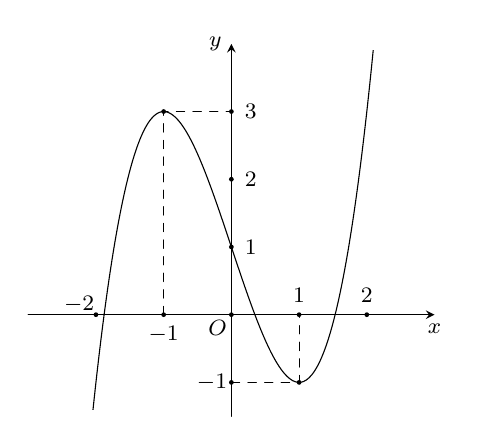
\begin{tikzpicture}[line join = round, line cap = round,>=stealth,font=\footnotesize,scale=.86]
\def\xt{-3} \def\xp{3} \def\yd{-1.5} \def\yt{4}
\def\a{1}
\def\b{0}
\def\c{-3}
\def\d{1}
\draw[->] (\xt,0)--(\xp,0) node[below]{$x$};
\draw[->] (0,\yd)--(0,\yt) node[left]{$y$};
\draw[dashed](-1,0)|-(0,3)(0,-1)-|(1,0);
\begin{scope}
\clip (\xt+0.1,\yd+0.1) rectangle (\xp-0.1,\yt-0.1);
\draw[samples=150,smooth,domain=\xt:\xp] plot(\x,{\a*(\x)^3+(\b)*(\x)^2+(\c)*\x+(\d)});
\end{scope}
\foreach \x/\y/\goc/\z in{-2/0/150/-2,-1/0/-90/-1,0/0/-135/O,1/0/90/1,2/0/90/2,0/-1/180/-1,0/1/0/1,0/2/0/2,0/3/0/3}
\fill (\x,\y)node[shift={(\goc:7pt)}]{$\z$}circle(1pt);
\fill(-1,3)circle(1pt)(1,-1)circle(1pt);
\end{tikzpicture}
}
\choice
{\True $3$}
{$5$}
{$6$}
{$2$}
\loigiai
{
\immini
{
Đặt $t=\cos x$ vì $x\in(0;\,\pi)$ nên $t\in(-1;1)$. Khi đó phương trình đã cho trở thành
\[f(t)-2m+1=2t \text{ với } t\in(-1;1)\quad(*).\]
Số nghiệm của phương trình $(*)$ bằng số giao điểm của hai đồ thị hàm số $y=f(t)$ và $y=2t+2m-1$ với $t\in(-1;1)$.\\
Các đường thẳng đi qua điểm $(-1;3)$, $(1;-1)$ và song song với đường thẳng $y=2t$ có phương trình lần lượt là $y=2t-3$ và $y=2t+5$.\\
Đường thẳng $y=2t-2m+1$, $y=2t-3$ và $y=2t+5$ cắt trục $Oy$ lần lượt tại $2m-1$, $-2$ và $5$.\\
Yêu cầu bài toán $\Leftrightarrow -3<2m-1<5\Leftrightarrow -1<m<3$.\\
Vì $m$ nguyên nên $m\in\{0;1;2\}$.\\
Vậy tổng các phần tử của $S$ là $0+1+2=3$.
}
{
\begin{tikzpicture}[line join = round, line cap = round,>=stealth,font=\footnotesize,scale=.86]
\def\xt{-3} \def\xp{3} \def\yd{-3.9} \def\yt{6.2}
\def\a{1}
\def\b{0}
\def\c{-3}
\def\d{1}
\draw[->] (\xt,0)--(\xp,0) node[below]{$x$};
\draw[->] (0,\yd)--(0,\yt) node[left]{$y$};
\draw[dashed](-1,0)|-(0,3)(0,-1)-|(1,0);
\foreach \x/\y/\goc/\z in{-2/0/150/-2,-1/0/-90/-1,0/0/-135/O,1/0/90/1,2/0/90/2,0/-1/180/-1,0/1/0/1,0/2/180/2,0/3/0/3,0/5/-45/5,0/-3/-45/-3,0/1.5/0/\quad\quad2m-1}
\fill (\x,\y)node[shift={(\goc:7pt)}]{$\z$}circle(1pt);
\fill(-1,3)circle(1pt)(1,-1)circle(1pt);
\draw(-2.5,0)--(0.5,6)
($(0,-3)!-0.2!(2,1)$)--($(2,1)!-0.2!(0,-3)$)
(-2,-2.5)--(1,3.5)
;
\begin{scope}
\clip (\xt+0.1,-1.5) rectangle (\xp-0.1,3.2);
\draw[samples=150,smooth,domain=\xt:\xp] plot(\x,{\a*(\x)^3+(\b)*(\x)^2+(\c)*\x+(\d)});
\end{scope}
\end{tikzpicture}
}
}
\end{ex}

\begin{ex}%[Đề thi KSCL lần 2 THPT Lê Xoay-Vĩnh Phúc năm 2023]%[Nguyễn Tấn Linh, dự án 12-EX-6-2023]%[2H3G2-4]
Trong không gian với hệ trục tọa độ $O x y z$, cho tứ diện $ABCD$ có điểm $A(1;-2;3)$, $B(5;0;-1)$, $C(-1;2;0)$, $D(0;3;4)$. Trên các cạnh $AB$, $AC$, $AD$ lần lượt lấy các điểm $M$, $N$, $P$ thỏa $\dfrac{AB}{AM}+\dfrac{AC}{AN}+\dfrac{AD}{AP}=9$ và có thể tích $AMNP$ nhỏ nhất. Khi đó mặt phẳng $(MNP)$ đi qua điểm nào sau đây?
\choice
{$\left(\dfrac{7}{3};\dfrac{4}{3};\dfrac{5}{3}\right)$}
{$\left(\dfrac{-27}{3};\dfrac{41}{3};\dfrac{5}{3}\right)$}
{$\left(\dfrac{5}{3};\dfrac{1}{3};\dfrac{74}{3}\right)$}
{\True $\left(\dfrac{1}{3};\dfrac{7}{3};\dfrac{91}{8}\right)$}
\loigiai
{
\immini
{
	\begin{eqnarray*}
		\dfrac{V_{A.BCD}}{V_{A.MNP}}&=&\dfrac{AB}{AM}\cdot\dfrac{AC}{AN}\cdot\dfrac{AD}{AP}\\
		&\le&\left(\dfrac{\dfrac{AB}{AM}+\dfrac{AC}{AN}+\dfrac{AD}{AP}}{3}\right)^3=\left(\dfrac{9}{3}\right)^3=27.
	\end{eqnarray*}
Suy ra $V_{A.MNP}\leq\dfrac{1}{27}V_{A.BCD}$.\\
Dấu bằng xảy ra khi $\dfrac{AB}{AM}=\dfrac{AC}{AN}=\dfrac{AD}{AP}=3$.
}
{
\begin{tikzpicture}[>=stealth,line join=round,line cap=round,font=\footnotesize,scale=1]
\coordinate (B) at (0,0);
\coordinate (C) at (1,-1);
\coordinate (D) at (4,0);
\coordinate (A) at (1.2,3);
\draw (B)--(C)--(D)--(A)--cycle (A)--(C)($(A)!1/3!(B)$)coordinate(M)--($(A)!1/3!(C)$)coordinate(N)--($(A)!1/3!(D)$)coordinate(P);
\draw[dashed] (B)--(D)($(A)!1/3!(B)$)--($(A)!1/3!(D)$);
\foreach \diem/\goc in {B/180,C/-90,D/0,A/90,M/150,N/-45,P/45} \fill[black](\diem) circle (1pt) ($(\diem)+(\goc:3mm)$) node{$\diem$};
\end{tikzpicture}
}
	\noindent Ta suy ra $(MNP)\parallel (BCD)$ và $\overrightarrow{AM}=\dfrac{1}{3}\overrightarrow{AB}$.\\
	Mặt khác $\heva{& \overrightarrow{AB}=(4;2;4) \\ & \overrightarrow{AM}=\dfrac{1}{3}\overrightarrow{AB}}\Rightarrow M\left(\dfrac{7}{3};-\dfrac{4}{3};\dfrac{5}{3}\right)$. Khi đó\\
	Mặt phẳng $(MNP)$ đi qua $M\left(\dfrac{7}{3};-\dfrac{4}{3};\dfrac{5}{3}\right)$ và có véc-tơ pháp tuyến là $\overrightarrow{n}=[\overrightarrow{BC},\overrightarrow{BD}]=(7;25;-8)$. Suy ra phương trình mặt phẳng $(MNP)$ là
	\[7x+25y-8z+\dfrac{91}{3}=0.\]
	Nhận xét $7\cdot \dfrac{1}{3}+25\cdot \dfrac{7}{3}-8\cdot\dfrac{91}{8}+\dfrac{91}{8}=0$.\\
	Suy ra mặt phẳng $(MNP)$ đi qua điểm $\left(\dfrac{1}{3}; \dfrac{7}{3}; \dfrac{91}{8}\right)$.
}
\end{ex}
\begin{ex}%[Đề thi KSCL lần 2 THPT Lê Xoay-Vĩnh Phúc năm 2023]%[Nguyễn Tấn Linh, dự án 12-EX-6-2023]%[2D3K2-4]
Cho hàm số $y=f(x)=\heva{&x^2+3&\text{ khi }&x\ge 1\\&5-x&\text{ khi }&x<1}$.\\
Tính $I=2\displaystyle\int\limits_0^{\frac{\pi}{2}} f(\sin x)\cos x\mathrm{\, d}x+\frac{3}{2}\displaystyle\int\limits_0^1f(3-2x)\mathrm{\, d}x$.
\choice
{$I=\dfrac{32}{3}$}
{\True $I=20$}
{$I=32$}
{$I=31$}
\loigiai
{
\begin{eqnarray*}
I&=&2\displaystyle\int\limits_0^{\frac{\pi}{2}} f(\sin x)\mathrm{\, d}(\sin x)+\frac{3}{2}\displaystyle\int\limits_0^1f(3-2x)\dfrac{\mathrm{\, d}(3-2x)}{-2}\\
&=&2\displaystyle\int\limits_0^1 f(x)\mathrm{\, d}x-\dfrac{3}{4}\displaystyle\int\limits_3^1 f(x)\mathrm{\, d}x=2\displaystyle\int\limits_0^1 f(x)\mathrm{\, d}x+\dfrac{3}{4}\displaystyle\int\limits_1^3 f(x)\mathrm{\, d}x\\
&=&2\displaystyle\int\limits_0^1 (5-x)\mathrm{\, d}x+\dfrac{3}{4}\displaystyle\int\limits_1^3 (x^2+3)\mathrm{\, d}x\\
&=&2\cdot\dfrac{9}{2}+\dfrac{3}{4}\cdot\dfrac{44}{3}\\
&=&20.
\end{eqnarray*}
}
\end{ex}

\begin{ex}%[Đề thi KSCL lần 2 THPT Lê Xoay-Vĩnh Phúc năm 2023]%[Nguyễn Tấn Linh, dự án 12-EX-6-2023]%[2H2K1-2]
\immini
{
Người ta sử dụng một cuộn đề can hình trụ có đường kính $64{,}9$ cm để in các băng rôn (tham khảo hình vẽ bên), khẩu hiệu chuẩn bị cho lễ ra quân năm $2023$, do đó đường kính của cuộn đề can còn lại là $8{,}2$ cm. Biết độ dày của tấm đề can là $0{,}04$ cm, hãy tính chiều dài $L$ của tấm đề can đã sử dụng? (Làm tròn đến hàng đơn vị).
\choice
{$L=325529$ cm}
{\True $L=81382$ cm}
{$L=7749$ cm}
{$L=24344$ cm}
}
{
\begin{tikzpicture}[>=stealth,line join=round,line cap=round,font=\footnotesize,scale=.9]
\draw[xslant=0.6,draw=none]
(1,0)circle(.39cm)
(1,0)circle(1cm)
($(1,0)+(60:1cm)$)--++(150:3cm)coordinate(C)
($(1,0)+(-130:1cm)$)coordinate (B)--++(150:3cm)coordinate(D)
($(1,0)+(60:1cm)$)coordinate (A) arc (60:180:1cm)
(C) arc (60:240:1cm)
;
\fill[xslant=0.6,outer color=gray!30,draw=none]
($(1,0)+(150:1cm)$)--++(150:3cm) arc (120:180:1cm)
(A) arc (60:240:1cm)--(B)--(D)arc(240:60:1cm)--cycle;
\fill[xslant=0.6,gray!70]
(1,0)circle(1cm);
\fill[xslant=0.6,white,inner color=gray!25]
(1,0)circle(.39cm);
\fill[xslant=0.6,gray,draw=none]($(1,0)+(150:1cm)$)--++(150:3.15cm) arc (120:180:1cm)--++(-30:3.15)--cycle;
\end{tikzpicture}
}
\loigiai
{
Bán kính đường tròn ban đầu $R=\dfrac{64{,}9}{2}=32{,}45$ cm.\\
Bán kính đường tròn còn lại $r=\dfrac{8{,}2}{2}=4{,}1$ cm.\\
Thể tích đã dùng $V=\pi\cdot h(R^2-r^2)$.\\
Chiều dài $L$ của tấm đề can đã sử dụng là
\[L=\dfrac{\pi(R^2-r^2)}{0{,}04}=\dfrac{\pi(32{,}45)-4{,}1}{0{,}04}=81382\text{ cm}.\]
}
\end{ex}

\begin{ex}%[Đề thi KSCL lần 2 THPT Lê Xoay-Vĩnh Phúc năm 2023]%[Nguyễn Tấn Linh, dự án 12-EX-6-2023]%[2D3K1-1]
\immini
{
Cho hàm số $y=f(x)$. Đồ thị của hàm số $y=f'(x)$ trên $[-5;3]$ như hình vẽ (phần cong của đồ thị là một phần của parabol $y=a x^2+b x+c$). Biết $f(0)=0$, giá trị của $2f(-5)+3f(2)$ bằng
\choice
{$33$}
{\True $\dfrac{35}{3}$}
{$11$}
{$\dfrac{109}{3}$}
}
{
\begin{tikzpicture}[line join = round, line cap = round,>=stealth,font=\footnotesize,scale=.7]
\def\xt{-5.5} \def\xp{4.5} \def\yd{-2} \def\yt{5}
\def\a{-1}
\def\b{2}
\def\c{3}
\draw[->] (\xt,0)--(\xp,0) node[below]{$x$};
\draw[->] (0,\yd)--(0,\yt) node[left]{$y$};
\fill (0,0) circle (1.5pt) node[above left]{$O$}(-5,-1)circle (1.5pt)(-4,2)circle (1.5pt)(1,4)circle (1.5pt)(2,3)circle (1.5pt);
\draw(-5,-1)--(-4,2)--(-1,0);
\draw[dashed](-5,0)|-(0,-1)(-4,0)|-(0,2)(0,4)-|(1,0)(0,3)-|(2,0);
\foreach \x/\y/\goc/\z in{-5/0/135/-5,-4/0/-90/-4,-1/0/-90/-1,1/0/-90/1,2/0/-90/2,3/0/45/3,0/-1/0/-1,0/2/0/2,0/3/180/3,0/4/180/4}
\fill (\x,\y)node[shift={(\goc:7pt)}]{$\z$}circle(1.5pt);
\begin{scope}
\clip (-1,-2) rectangle (\xp-0.1,\yt-0.1);
\draw[samples=100,domain=\xt:\xp,smooth] plot (\x, {\a*(\x)^2+(\b)*\x+(\c)});
\end{scope}
\end{tikzpicture}
}
\loigiai
{
Từ đồ thị của $f'(x)$ ta suy ra
\begin{eqnarray*}
&&f'(x)=\heva{& 3x+14&\text{khi }&-5<x\leq -4 \\ & -\dfrac{2}{3}x-\dfrac{2}{3}&\text{khi }&-4<x\leq -1\\ & -x^2+2x+3&\text{khi }&-1<x<3.}\\
&&f(x)=\heva{& \dfrac{3}{2}x^2+14x+C_1&\text{khi }&-5<x\leq -4 \\ & -\dfrac{1}{3}x^2-\dfrac{2}{3}x+C_2&\text{khi }&-4<x\leq -1\\ & -\dfrac{1}{3}x^3+x^2+3x+C_3&\text{khi }&-1<x<3.}
\end{eqnarray*}
Ta có $f(0)=0\Leftrightarrow C_3=0$.\\
Hàm số $f(x)$ lên tục tại $x=-1\Rightarrow \lim \limits_{x \to -1^-} f(x)=\lim \limits_{x \to -1^+} f(x)\Leftrightarrow \dfrac{1}{3}+C_2=-\dfrac{5}{3}\Leftrightarrow C_2=-2$.\\
Hàm số liện tục tại $x=-4\Rightarrow \lim \limits_{x \to -4^-} f(x)=\lim \limits_{x \to -4^+} f(x)\Leftrightarrow -32+C_1=-\dfrac{14}{3}\Leftrightarrow C_1=\dfrac{82}{3}$.\\
Vậy $2f(-5)+3f(2)=2\cdot \left(-\dfrac{31}{6}\right)+3\cdot \dfrac{22}{3}=\dfrac{35}{3}$.
}
\end{ex}
\begin{ex}%[Đề thi KSCL lần 2 THPT Lê Xoay-Vĩnh Phúc năm 2023]%[Nguyễn Tấn Linh, dự án 12-EX-6-2023]%[2D1G1-3]
Có bao nhiêu số nguyên $m$ thuộc khoảng $(-2023;2023)$ để hàm số $y=\left|2x^3-2m x+3\right|$ đồng biến trên $(1;+\infty)$?
\choice
{$2023$}
{$2025$}
{\True $12$}
{$4042$}
\loigiai
{
Xét hàm số $f(x)=2x^3-2mx+3$ trên $(1;\infty)$.\\
Ta có $f'(x)=6x^2-2m$. Khi đó $\Delta=48m$.\\
Để hàm số $y=|2x^3-2mx+3|$ đồng biến trên $(1;+\infty)$ thì ta xét hai trường hợp sau\\
\textbf{TH1:} $\Delta\leq 0\Leftrightarrow 48m\leq 0\Leftrightarrow m\leq 0\Rightarrow f'(x)\geq 0$, $\forall x\in(1;+\infty)$.\\
Yêu cầu bài toán $\Leftrightarrow\heva{& m\leq 0 \\ & f(1)\geq 0}\Leftrightarrow\heva{& m\leq 0 \\ & 5-2m\geq 0}\Leftrightarrow\heva{& m\leq 0 \\ & m\leq \dfrac{5}{2}}\Leftrightarrow m\leq 0$.\\
Vì $m\in\mathbb{Z}$ và $m\in(-10;10)$ nên $m\in\{-9;-8;-7;-6;-5;-4;-3;-2;-1;0\}$\quad$(1)$.\\
\textbf{TH2:} $\Delta>0\Leftrightarrow m>0$.\\
Suy ra $f'(x)=0$ có 2 nghiệm phân biệt $x_1$, $x_2\quad\left(x_1<x_2\right)$.\\
Ta có bảng biến thiên
\begin{center}

\begin{tikzpicture}[>=stealth]
\tkzTabInit[nocadre=false,lgt=1,espcl=3,deltacl=0.5]{$x$/.7 ,$y'$/.7,$y$/2}
{$-\infty$ , $x_1$ , $x_2$ , $+\infty$}
\tkzTabLine{ , + , $0$ , - , $0$ , + , }
\tkzTabVar{-/$-\infty$ , +/$f(x_1)$ , -/$f(x_2)$ , +/$+\infty$}
\end{tikzpicture}
\end{center}
Vậy yêu cầu bài toán
\[\Leftrightarrow\heva{&m>0\\&x_1<x_2\leq 1\\&f(1)\geq 0}\Leftrightarrow\heva{&m>0\\&-\dfrac{2m}{6}+1\geq 0\\&5-2m\geq 0}\Leftrightarrow  0<m\leq\dfrac{5}{2}\Leftrightarrow 5-2m\geq 0.\]
Vì $m\in\mathbb{Z}$ và $m\in(-10;10)$ nên $m\in\{1;2\}$\quad$(2)$.\\
Từ $(1)$ và $(2)$ suy ra có tất cả $12$ giá trị của $m$ thỏa mãn yêu cầu bài toán.
}
\end{ex}

\begin{ex}%[Đề thi KSCL lần 2 THPT Lê Xoay-Vĩnh Phúc năm 2023]%[Nguyễn Tấn Linh, dự án 12-EX-6-2023]%[2D2G6-2]
Gọi $S$ là tập hợp tất cả các giá trị thực của $m$ để tồn tại duy nhất cặp số $(x;y)$ thỏa mãn $\log_{x^2+y^2+2}\left(4x+4y+m^2-6m+3\right)\ge 1$ và $x^2+y^2+2x-4y+1=0$. Tổng giá trị các phần tử của tập $S$ bằng
\choice
{$12$}
{\True $0$}
{$6$}
{$8$}
\loigiai
{
Ta có
\begin{eqnarray*}
&&\log _{x^2+y^2+2}\left(4 x+4 y-6+m^2\right) \geq 1\\
&\Leftrightarrow&\log _{x^2+y^2+2}\left(4 x+4 y-6+m^2\right)\geq\log _{x^2+y^2+2}\left(x^2+y^2+2\right)\\
&\Leftrightarrow&4x+4y-6+m^2 \geq x^2+y^2+2\quad\left(\text{Do } x^2+y^2+2>1\right)\\
&\Leftrightarrow&x^2+y^2-4x-4y-m^2+8 \leq 0.
\end{eqnarray*}
Ta có $a^2+b^2-c=4+4+m^2-8=m^2$\quad$(2)$.\\
\textbf{TH1:} $m=0\Rightarrow(1): x^2+y^2-4x-4y+8=0\Leftrightarrow(x-2)^2+(y-2)^2=0\Leftrightarrow\heva{&x=2\\&y=2.}$\\
Cặp số $(x;y)=(2;2)$ không thỏa mãn điều kiện $(2)$.\\
\textbf{TH2:} $m\neq 0\Rightarrow m^2>0\Rightarrow$. Tập hợp các cặp số $(x;y)$ thỏa mãn $(1)$ là hình tròn $(C_1)$ (kể cả biên) tâm $I_1(2;2)$ bán kính $R_1=m$.\\
Tập hợp các cặp số $(x;y)$ thôa màn $(2)$ là đường tròn $(C_2)$ có tâm $I_2(-1;2)$, bán kính $R_2=\sqrt{1+4-1}=2$. Để tồn tại duy nhất cặp số $(x;y)$ thỏa mãn $2$ điều kiện $(1)$ và $(2)\Rightarrow$ xảy ra 2 trường hợp sau
\begin{itemize}
\item \textbf{TH1:} $(C_1)$ và $(C_2)$ tiếp xúc ngoài
\begin{eqnarray*}
&\Leftrightarrow& I_1 I_2=R_1+R_2\\ &\Leftrightarrow&\sqrt{(-1-2)^2+(2-2)^2}=m+2\\
&\Leftrightarrow& 3=m+2 \Leftrightarrow m=1\quad\text{(thỏa mãn)}.
\end{eqnarray*}
\item \textbf{TH2:} $(C_1)$ và $(C_2)$ tiếp xúc trong và $R_1<R_2$
\begin{eqnarray*}
&\Leftrightarrow& \heva{&{I_1 I_2=|R_1-R_2|}\\&{m<2}}\Leftrightarrow\heva{&3=|m-2|\\&m<2}\\
&\Leftrightarrow&\heva{&\hoac{&m=5\\&m=-1}\\&m<2}\\
&\Leftrightarrow&m=-1\quad(\text{thỏa mãn}).
\end{eqnarray*}
\end{itemize}
Vậy $S=\{-1;1\}\Rightarrow$ Tổng giá trị các phần tử của tập $S$ bằng $0$.
}
\end{ex}
\Closesolutionfile{ans}
\begin{indapan}{10}
{ans/ans-2-TT-31-KSCL-LeXoay-VinhPhuc-23}
\end{indapan}